
    
    
    
    

%~\par
%\newpage 

    

    % No prompt!
%\textbf{Input \#{}}%
\begin{lstlisting}
%%javascript 
IPython.load_extensions('calico-document-tools');
\end{lstlisting}% No prompt!
%\textbf{Output \#{}}
%
    
    \begin{verbatim}
<IPython.core.display.Javascript object>
    \end{verbatim}

    % No prompt!
%\textbf{Input \#{}}%
\begin{lstlisting}
%%javascript 
IPython.load_extensions('latex_envs');
\end{lstlisting}% No prompt!
%\textbf{Output \#{}}
%
    
    \begin{verbatim}
<IPython.core.display.Javascript object>
    \end{verbatim}

    % No prompt!
%\textbf{Input \#{}}%
\begin{lstlisting}
%%html
<style>
    .prompt{
        display: none;
    }    

</style>
\end{lstlisting}
    \section{Goal}\label{goal}

    \subsection{Initial goal}\label{initial-goal}

    The initial goal was only to add an environment \texttt{theorem} in my
workflow. That is to be able to type something like

\begin{listing}
\begin{theorem}
Let $u$ and $v$ be two vectors of $\mathbb{R}^n$. The dot product can be
expressed as \begin{equation}u^Tv = |u||v| \cos \theta,\end{equation} where $\theta$ is the angle
between $u$ and $v$ \ldots{}
\end{theorem}
\end{listing}

in a markdown cell and have it rendered, like

\begin{theorem}
Let $u$ and $v$ be two vectors of $\mathbb{R}^n$. The dot product can be
expressed as \begin{equation}u^Tv = |u||v| \cos \theta,\end{equation} where $\theta$ is the angle
between $u$ and $v$ \ldots{}
\end{theorem}

    \subsection{Features}\label{features}

    The initial project has evolved to account for more environments and
introduce some other features.

    \subsubsection{Support for simple LaTeX
commands}\label{support-for-simple-latex-commands}

    We also added some LaTeX commands (e.g. \texttt{\textbackslash{}textit},
\texttt{\textbackslash{}textbf}, \texttt{\textbackslash{}underline}) --
this is useful in the case of copy-paste from a LaTeX document. Labels
and references are supported, including for equations.

    \subsubsection{Available environments}\label{available-environments}

    \begin{itemize}
\itemsep1pt\parskip0pt\parsep0pt
\item
  \textbf{theorems-like environments}: \emph{property, theorem, lemma,
  corollary, proposition, definition,remark, problem, exercise,
  example},
\item
  \textbf{lists}: \emph{enumerate, itemize},\\
\item
  limited support for a \emph{figure} environment,
\item
  an environment \emph{listing},
\item
  \emph{textboxa}, wich is a \texttt{textbox} environment defined as a
  demonstration (see below).
\end{itemize}

More environments can be added easily in the javascript source file
\texttt{thmsInNb.js}. The rendering is done according to the stylesheet
\texttt{latex\_env.css}, which can be customized.

    \subsubsection{Automatic numerotation}\label{automatic-numerotation}

    Counters for numbering are implemented: one for theorems-like
environments, a second for exercises-like environments and a third one
for numbering figures.\\Mathjax-equations with a label are also numbered
document-wide (in contrast with standard notebook/mathjax numbering
where the scope of numbering is limited to cells). An anchor is created
for any label which enables to links things in the document:
\texttt{\textbackslash{}label} and \texttt{\textbackslash{}ref} are both
supported. A limitation is that numbering is updated (incremented) each
time a cell is rendered. A toolbar button is provided to reset the
counters and refresh the rendering of the whole document.

    \subsubsection{Other features}\label{other-features}

    \begin{itemize}
\itemsep1pt\parskip0pt\parsep0pt
\item
  It is possible to mix LaTeX and markdown markup in environments\\
\item
  Environments can be nested. However, this is not always
  perfect\ldots{}
\end{itemize}

    \section{Usage and examples}\label{usage-and-examples}

    \subsection{Installation}\label{installation}

    The extension consists in two javascript scripts:
\texttt{latex\_envs.js}, \texttt{thmsInNb.js} together with a stylesheet
\texttt{latex\_envs.css}. Follow the instructions in the
\href{https://github.com/ipython-contrib/IPython-notebook-extensions/wiki}{wiki}
to install the extension. You can simply copy these files in the
notebook extension directory (usually
\textasciitilde{}/.ipython/nbextensions) and load the extension in the
notebook by

\begin{verbatim}
%%javascript 
IPython.load_extensions('latex_envs');
\end{verbatim}

    \subsection{A first example}\label{a-first-example}

    This example shows another example of environment, featuring automatic
numerotation, and the use of labels and references. Also note that
standard markdown can be present in the environment and is interpreted.
\emph{The rendering is done according to the stylesheet
\texttt{latex\_env.css}, which of course, can be tailored to specific
uses and tastes}.

    \begin{listing}
\begin{definition}
\label{def:FT} Let $x[n]$ be a sequence of length $N$. Then, its
\textbf{Fourier transform} is given by

\begin{equation}
\label{eq:FT}
X[k]= \frac{1}{N} \sum_{n=0}^{N-1} x[n] e^{-j2\pi \frac{kn}{N}}
\end{equation}
\end{definition}
\end{listing}

    \begin{definition}
\label{def:FT} Let $x[n]$ be a sequence of length $N$. Then, its
\textbf{Fourier transform} is given by

\begin{equation}
\label{eq:FT2}
X[k]= \frac{1}{N} \sum_{n=0}^{N-1} x[n] e^{-j2\pi \frac{kn}{N}}
\end{equation}
\end{definition}

    This is an extremely important tool in signal processing. We put this in
evidence using the \texttt{textboxa} environment -- which is defined
here in the css, and that one should define in the LaTeX counterpart:

\begin{listing}
\begin{textboxa}
The Fourier transform is an extremely useful tool to have in your toolbox!
\end{textboxa}
\end{listing}

    \begin{textboxa}
The Fourier transform is an extremely useful tool to have in your toolbox!
\end{textboxa}

    As an example, consider the Fourier transform (\ref{eq:FT2}) of a pure
cosine wave given by \begin{equation}
x[n]= \cos(2\pi k_0 n/N),
\end{equation} where $k_0$ is an integer. Its Fourier transform is given by \begin{equation}
X[k] = \frac{1}{2} \left( \delta[k-k_0] + \delta[k-k_0] \right), 
\end{equation} modulo $N$. This is illustrated in the following simple script:
% No prompt!
%\textbf{Input \#{}}%
\begin{lstlisting}
%matplotlib inline
import numpy as np
import matplotlib.pyplot as plt 
from numpy.fft import fft
k0=4; N=128; n=np.arange(N); k=np.arange(N)
x=np.sin(2*np.pi*k0*n/N)
X=fft(x)
plt.stem(k,np.abs(X))
plt.xlim([0, 20])
plt.title("Fourier transform of a cosine")
_=plt.xlabel("Frequency index (k)")
\end{lstlisting}% No prompt!
%\textbf{Output \#{}}
%
    \begin{center}
    \adjustimage{max size={0.6\linewidth}{0.6\paperheight}}{latex_env_doc_tmp_files/latex_env_doc_tmp_26_0.png}
    \end{center}
%    { \hspace*{\fill} \\}
    
    \subsection{Second example}\label{second-example}

    This example shows a series of environments, with different facets;
\textbf{links, references, markdown or/and LaTeX formatting within
environments}. Again, the rendering is done according to the stylesheet
\texttt{latex\_env.css}, which can be tailored. The listing of
environments below is typed using the environment \emph{listing}\ldots{}

    \begin{listing}
\begin{definition}
\label{def:diffeq} We call \textbf{difference equation} an equation of
the form \begin{equation}
\label{eq:diffeq}
y[n]= \sum_{k=1}^{p} a_k y[n-k] + \sum_{i=0}^q b_i x[n-i]
\end{equation}
\end{definition}

\begin{property}
If all the $a_k$ in equation (\ref{eq:diffeq}) of definition
\ref{def:diffeq} are zero, then the filter has a \textbf{finite impulse
response}.
\end{property}

\begin{proof}
Let $\delta[n]$ denote the Dirac impulse. Take $x[n]=\delta[n]$ in
(\ref{eq:diffeq}). This yields, by definition, the impulse response: \begin{equation}
\label{eq:fir}
h[n]= \sum_{i=0}^q b_i \delta[n-i],
\end{equation} which has finite support.
\end{proof}

\begin{theorem}
The poles of a causal stable filter are located within the unit circle
in the complex plane.
\end{theorem}

\begin{example}
\label{ex:IIR1} Consider $y[n]= a y[n-1] +  x[n]$. The pole of the
transfer function is $z=a$. The impulse response $h[n]=a^n$ has infinite
support.
\end{example}

In the following exercise, you will check that the filter is stable iff $a$<1.

\begin{exercise}
\label{ex:exofilter} Consider the filter defined in Example
\ref{ex:IIR1}. Using the \textbf{function} \texttt{lfilter} of scipy,
compute and plot the impulse response for several values of $a$.
\end{exercise}

\end{listing}

    The lines above are rendered as follows (of course everything can be
tailored in the stylesheet):

\begin{definition}
\label{def:diffeq} We call \textbf{difference equation} an equation of
the form

\begin{equation}
\label{eq:diffeq}
y[n]= \sum_{k=1}^{p} a_k y[n-k] + \sum_{i=0}^q b_i x[n-i]
\end{equation}
\end{definition}

Properties of the filter are linked to the coefficients of the
difference equation. For instance, an immediate property is

\begin{property}
If all the $a_k$ in equation (\ref{eq:diffeq}) of definition
\ref{def:diffeq} are zero, then the filter has a \textbf{finite impulse
response}.
\end{property}

\begin{proof}
Let $\delta[n]$ denote the Dirac impulse. Take $x[n]=\delta[n]$ in
(\ref{eq:diffeq}). This yields, by definition, the impulse response:

\begin{equation}
\label{eq:fir}
h[n]= \sum_{i=0}^q b_i \delta[n-i],
\end{equation}

which has finite support.
\end{proof}

\begin{theorem}
The poles of a causal stable filter are located within the unit circle
in the complex plane.
\end{theorem}

\begin{example}
\label{ex:IIR1} Consider $y[n]= a y[n-1] +  x[n]$. The pole of the
transfer function is $z=a$. The impulse response $h[n]=a^n$ has infinite
support.
\end{example}

In the following exercise, you will check that the filter is stable iff
$a$\textless{}1.

\begin{exercise}
\label{ex:exofilter} Consider the filter defined in Example
\ref{ex:IIR1}. Using the \textbf{function} \texttt{lfilter} of scipy,
compute and plot the impulse response for several values of $a$.
\end{exercise}

    \begin{listing}
The solution of exercise \ref{ex:exofilter}, which uses a difference equation as in Definition \ref{def:diffeq}:
\end{listing}

The solution of exercise \ref{ex:exofilter}, which uses a difference
equation as in Definition \ref{def:diffeq}:
% No prompt!
%\textbf{Input \#{}}%
\begin{lstlisting}
%matplotlib inline
import numpy as np
import matplotlib.pyplot as plt 
from scipy.signal import lfilter
d=np.zeros(100); d[0]=1 #dirac impulse
alist=[0.2, 0.8, 0.9, 0.95, 0.99, 0.999, 1.001, 1.01]
for a in alist:
    h=lfilter([1], [1, -a],d)
    _=plt.plot(h, label="a={}".format(a))
plt.ylim([0,1.5])
plt.xlabel('Time')
_=plt.legend()
\end{lstlisting}% No prompt!
%\textbf{Output \#{}}
%
    \begin{center}
    \adjustimage{max size={0.6\linewidth}{0.6\paperheight}}{latex_env_doc_tmp_files/latex_env_doc_tmp_32_0.png}
    \end{center}
%    { \hspace*{\fill} \\}
    
    Finally, it is sometimes useful to integrate a figure within a markdown
cell. The standard markdown markup for that is
\texttt{!{[}link{]}(image)}, but a limitation is that the image can not
be resized, can not be referenced and is not numbered. Furthermore it
can be useful to re-use existing code. Threfore we have added a limited
support for the \texttt{figure} environment. This enables to do
something like

\begin{listing}
\begin{figure}[H]
\centerline{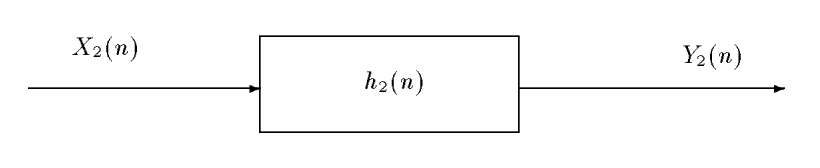
\includegraphics[width=10cm]{example.png}}
\caption{\label{fig:example} This is an example of figure included using LaTeX commands.}
\end{figure}
\end{listing}

which renders as

\begin{figure}[H]
\centerline{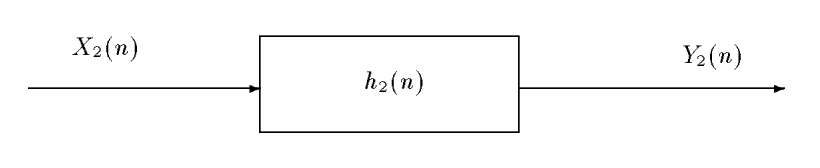
\includegraphics[width=10cm]{example.png}}
\caption{\label{fig:example} This is an example of figure included using LaTeX commands.}
\end{figure}

Of course, this Figure can now be referenced:

\begin{listing}
Figure \ref{fig:example} shows a second filter with input $X_2$, output $Y_2$  and an impulse response denoted as $h_2(n)$
\end{listing}

Figure \ref{fig:example} shows a second filter with input $X_2$, output
$Y_2$ and an impulse response denoted as $h_2(n)$

    \subsection{Third example:}\label{third-example}

    This example shows that environments like itemize or enumerate are also
available. As already indicated, this is useful for copying text from a
TeX file. Following the same idea, text formating commands
\texttt{\textbackslash{}textit}, \texttt{\textbackslash{}textbf},
\texttt{\textbackslash{}underline}, etc are also available.

    \begin{listing}
The following \textit{environments} are available:
\begin{itemize}
    \item \textbf{Theorems and likes}
    \begin{enumerate}
        \item theorem,
        \item lemma,
        \item corollary
        \item ...
    \end{enumerate}
    \item \textbf{exercises}
    \begin{enumerate}
        \item problem,
        \item example,
        \item exercise
    \end{enumerate}
\end{itemize}
\end{listing}

    which gives\ldots{}

The following \textit{environments} are available:

\begin{itemize}
\item \textbf{Theorems and likes}
\begin{enumerate}
\item theorem,
\item lemma,
\item corollary
\item ...
\end{enumerate}
\item \textbf{exercises}
\begin{enumerate}
\item problem,
\item example,
\item exercise
\end{enumerate}
\end{itemize}

    \section{(post)-Converters}\label{post-converters}

    The extension works in the live-notebook. Since it relies on a bunch of
javascript, the notebook does not render as is in very nice services
such as \texttt{nbviewer} or \texttt{github} viewer. Similarly,
\texttt{nbconvert} does not know of the LaTeX constructs which are used
and therefore do not fully convert notebooks making use of this
extension. Therefore, it is necessary to add a post conversion step to
conversions provided by \texttt{nbconvert}. Though an interface exists
for adding post-converters to nbconvert, this (first) author was too
lazy and not enough strong to implement the post conversion along these
lines. What has be done are simple \texttt{bash} and \texttt{python}
scripts that perform this conversion.

    \subsection{Installation}\label{installation}

    Copy the scripts files to a directory in your search path, or launch the
scripts with the complete path. The two main scripts are
\texttt{ipynb\_thms\_to\_html} (conversion to html, of course:) and
\texttt{ipynb\_thms\_to\_latex} (conversion to LaTeX!).

    \subsection{Conversion to html}\label{conversion-to-html}

    \textbf{Requirements}: You will need \texttt{perl}, \texttt{nodejs}, and
\texttt{ipython3} (the script calls \texttt{ipython3}; if your
interpreter is \texttt{ipython}, edit the script and replace the
different occurences).

The conversion to html is done by something like

\begin{verbatim}
    [path/]ipynb_thms_to_html filename
\end{verbatim}

or a list of files such as

\begin{verbatim}
    [path/]ipynb_thms_to_html *.ipynb
\end{verbatim}

In turn, this script makes somes substitutions using \texttt{perl}, and
then uses the \texttt{nodesj} javascript interpreter to make the very
same substitutions that are done in the live notebook. The conversion
uses the template \texttt{thmsInNb.tpl} (located in the script
directory). It also copies the css \texttt{latex\_env.css} in the
directory of the output html file (it must be copied with html files in
the case of web upload).

    \subsection{Conversion to LaTeX}\label{conversion-to-latex}

    \textbf{Requirements}: You will need \texttt{perl} and
\texttt{ipython3}.

The conversion to LaTeX is done by something like

\begin{verbatim}
    [path/]ipynb_thms_to_latex filename
\end{verbatim}

or a list of files such as

\begin{verbatim}
    [path/]ipynb_thms_to_latex *.ipynb
    
\end{verbatim}

The script makes some substitutions and cleaning in arkdown cells, then
calls the legacy \texttt{nbconvert}. Afterward, it runs through the
LaTeX environments and converts their contents (which can contain
markdown markup) to LaTeX. Note that the script contains a list of the
LaTeX environments to process. In the case of the addition of an
environment in the main javascript (\texttt{thmsInNb.js}), this list
must also be updated.

Finally, the script removes the header and footer in the LaTeX file.
This is a personnal choice, and the corresponding line can be safely
commented.

\begin{example}
As for an example, the present document has been converted using

\begin{verbatim}
ipynb_thms_to_latex latex_env_doc.ipynb
\end{verbatim}

Then the resulting file (without header/footer) has been included in the
main file \texttt{documentation.tex}, where some LaTeX definitions of
environments are done (namely listings, colors, etc) and compiled using

\begin{verbatim}
xelatex documentation
\end{verbatim}

The output can be consulted \href{documentation.pdf}{here}.
\end{example}

    \section{Disclaimer, sources and
thanks}\label{disclaimer-sources-and-thanks}

    This is a not-quick but certainly dirty hack. I am a complete beginner
in javascript and of course there are obviously a large amount of
possible improvements of the code, in cleaning, factorizing, etc!
Language also needs improvement.

\textbf{Contributions will be welcome and deeply appreciated.}

Originally, I used a piece of code from the nice online markdown editor
\texttt{stackedit}
\url{https://github.com/benweet/stackedit/issues/187}, where the authors
also considered the problem of incorporating LaTeX markup in their
markdown. I also used examples and code from
\url{https://github.com/ipython-contrib/IPython-notebook-extensions}.
% No prompt!
%\textbf{Input \#{}}%
\begin{lstlisting}
%%javascript 
IPython.load_extensions('latex_envs');
\end{lstlisting}% No prompt!
%\textbf{Output \#{}}
%
    
    \begin{verbatim}
<IPython.core.display.Javascript object>
    \end{verbatim}

    

    % Add a bibliography block to the postdoc
    
    
%\bibliographystyle{ieetran}
%\bibliography{Thesis}

    
    